%; whizzy chapter -dvi
% -initex iniptex -latex platex -format platex -bibtex jbibtex -fmt fmt
% 以上 whizzytex を使用する場合の設定。
 
%     Tokyo Debian Meeting resources
%     Copyright (C) 2012 Junichi Uekawa
%     Copyright (C) 2011 Nobuhiro Iwamatsu

%     This program is free software; you can redistribute it and/or modify
%     it under the terms of the GNU General Public License as published by
%     the Free Software Foundation; either version 2 of the License, or
%     (at your option) any later version.

%     This program is distributed in the hope that it will be useful,
%     but WITHOUT ANY WARRANTY; without even the implied warranty of
%     MERCHANTABILITY or FITNESS FOR A PARTICULAR PURPOSE.  See the
%     GNU General Public License for more details.

%     You should have received a copy of the GNU General Public License
%     along with this program; if not, write to the Free Software
%     Foundation, Inc., 51 Franklin St, Fifth Floor, Boston, MA  02110-1301 USA

%  preview (shell-command (concat "evince " (replace-regexp-in-string "tex$" "pdf"(buffer-file-name)) "&"))

%%ここからヘッダ開始。

\documentclass[mingoth,a4paper]{jsarticle}
\usepackage{monthlyreport}
% 日付を定義する、毎月変わります。
\newcommand{\debmtgyear}{2013}
\newcommand{\debmtgmonth}{12}
\newcommand{\debmtgdate}{21}
% started from zero:
% (let ((year 2013) (month 7)) (+ (* (- year 2005) 12) month -1))
\newcommand{\debmtgnumber}{107}

% ルビ
\def\ruby#1#2{%
\leavevmode
\setbox0=\hbox{#1}\setbox1=\hbox{\tiny#2}%
\ifdim\wd0>\wd1 \dimen0=\wd0 \else \dimen0=\wd1 \fi
\hbox{\kanjiskip=\fill
\vbox{\hbox to \dimen0{\tiny \hfil#2\hfil}%
\nointerlineskip
\hbox to \dimen0{\hfil#1\hfil}}}}

\begin{document}

\begin{titlepage}
\thispagestyle{empty}
% タイトルページ:編集必要な部分は最初のマクロに飛ばすこと

\vspace*{-2cm}
第\debmtgnumber{}回 東京エリア Debian 勉強会資料\\
\hspace*{-2cm}

\includegraphics{image2012-natsu/dotdeb.pdf}\\
\hfill{}\debmtgyear{}年\debmtgmonth{}月\debmtgdate{}日

% ここはアップデートすること
% 全角文字にしないとフォントのサイズが合わないので注意
\rotatebox{10}{\fontsize{32}{32} {\gt 特集1: 2013年の振り返り}}\\
\rotatebox{10}{\fontsize{32}{32} {\gt 特集2: GNU/Hurd 2013}}

\vspace*{-2cm}
\hfill{}
\includegraphics[height=6cm]{image200502/openlogo-nd.eps}
\end{titlepage}

\newpage

\begin{minipage}[b]{0.2\hsize}
 \definecolor{titleback}{gray}{0.9}
 \colorbox{titleback}{\rotatebox{90}{\fontsize{80}{80} {\gt デビアン勉強会} }}
\end{minipage}
\begin{minipage}[b]{0.8\hsize}
\hrule
\vspace{2mm}
\hrule
\begin{multicols}{2}
\tableofcontents
\end{multicols}
\vspace{2mm}
\hrule
\end{minipage}

\dancersection{事前課題}{野島 貴英}

今回の事前課題は以下です:
\begin{enumerate}
 \item 来年の東京エリアDebian勉強会の開催形式について妄想ください。(回答例:セミナ形式+ハッカソン形式で、〜をやるぞーなど)
\end{enumerate}
この課題に対して提出いただいた内容は以下です。
\begin{multicols}{2}
{\small
 \begin{prework}{ 河本拓 }

 インタビュー形式で、参加者のみなさんが「オープンソースに関わったきっかけ」などのお話が聞けたら嬉しいです。2014年最初の勉強会だと思うので、新年の抱負などと合わせて...(?)
\\
追記:初参加です。Linux初心者ですがよろしくお願いします。
\end{prework}

\begin{prework}{ dictoss(杉本 典充) }

基本的にはハックカフェのようにdebianに関する作業をする場として集まり、質問や議論があれば集まった人たちの中で話す、という場を提供することにするとよさそう。
参加の条件として行った作業や成した事、成せなかった事をまとめてブログ記事を必ず1つその場で書くこととする、というのはどうだろうか。そのとき各個人のブログサイトではなく、「勉強会ブログ」のようなサイトで一元的に記事を登録するようにして、対外的にdeibanのトレンドを発信することも兼ねるというのはどうだろうか。
ただ参加者の間でパッケージやdebianの仕組みについて勉強会が必要と判断することもあるので、その場合はセミナー形式で開催すればいいと思う。
\end{prework}

\begin{prework}{ 吉野(yy\_{}y\_{}ja\_{}jp) }

特に変わらないと思っていました
\end{prework}

\begin{prework}{ 野島 貴英 }

原稿/プレゼン集まればセミナー形式、集まらなければ、ハッカソン(作業時間)にするのがよいかなー?とりあえず、来年こそは、debian組み込みネタか、ハードウェアネタをやりたい。
\end{prework}

}
\end{multicols}

\dancersection{Debian Trivia Quiz}{野島 貴英}

ところで、みなさん Debian 関連の話題においついていますか?Debian関連の話
題はメーリングリストをよんでいると追跡できます。ただよんでいるだけではは
りあいがないので、理解度のテストをします。特に一人だけでは意味がわからな
いところもあるかも知れません。みんなで一緒に読んでみましょう。

今回の出題範囲は\url{debian-devel-announce@lists.debian.org} や \url{debian-devel@lists.debian.org}に投稿された
内容などからです。

\begin{multicols}{2}
%; whizzy-master ../debianmeetingresume201311.tex
% $B0J>e$N@_Dj$r$7$F$$$k$?$a!"$3$N%U%!%$%k$G(B M-x whizzytex $B$9$k$H!"(Bwhizzytex$B$,MxMQ$G$-$^$9!#(B
%

\santaku
{2013/12/15$B$K=P$?(BDebian wheezy$B$N%"%C%W%G!<%H$N%P!<%8%g%s$O!)(B}
{7.3}
{7.2}
{7.1}
{A}
{debian wheezy$B$r$*;H$$$N3'MM$OAaB.%"%C%W%G!<%H$7$^$7$g$&!*(B}

\santaku
{Debian$B$b;22C$7$F$$$k(BFOSS$B9W8%<T$K=w@-$rA}$d$=$&1?F0$N;v$r$J$s$H$$$&!)(B}
{Encourage Women in Linux}
{Outreach Program For Women}
{IT$B@o;N(B}
{B}
{Outreach Program For Women($BN,$7$F(BOPW)$B$O!"(B\\
\url{http://gnome.org/opw/}
$B$K>pJs$,$"$j$^$9!#(B}

\santaku
{$B@hF|(BDebian$B$N(BTechnical Committee$B$K%a%s%P$,A}$($^$7$?!#$H$3$m$G!"(B
 $B8=:_$N(BTechnical Comittee$B$N(Bchair man$B$OC/$G$7$g$&(B?}
{Takahide Nojima}
{Lucas Nussbaum}
{Bdale Garbee}
{C}
{$B85(BHP$B$N(BLinux$BItLg$N(BCTO$B$rL3$a$?$H$$$&7PNr$N;}$A<g$G$9!#(Bdebconf$B$H$+$K(B
$B;22C(B/$B%S%G%*;kD0$H$+$9$k$H$o$+$k$N$G$9$,!">oO"$5$s$N$h$&$G$9!#(B}


\end{multicols}

\dancersection{最近のDebian関連のミーティング報告}{野島 貴英}

\subsection{東京エリアDebian勉強会106回目報告}

 東京エリアDebian勉強会106回めは杉並区荻窪で開催されました。
8名の参加者がありました。

\begin{itemize}
\item 野島さんが、debian sidでのwaylandの動かし方、内部構造、周辺技術の紹介を行いました。また、KMS/DRM(i810ドライバ)を使い、X無しにて、実際にwaylandを動かし、プロジェクタに出力してwaylandのデモを行いました。
\item 上川さんが、emacs上で動く、リモート環境のファイル操作に関する拡張のtrampについてデモと説明を行いました。
\end{itemize}

 全体としてハックに活用できるネタが多かった印象でした。
 
 宴会は「はなの舞」にて行いました。
 

% % (query-replace-regexp "<.*?>" "")
% % (query-replace-regexp "^[	 ]\+" "")

%-------------------------------------------------------------------------------
\dancersection{2013年東京エリアDebian勉強会の振り返り}{野島 貴英}
%-------------------------------------------------------------------------------
\index{2013review}

\subsection{はじめに}

 2013年の東京エリアDebian勉強会を振り返ってみる企画です。
 毎年アンケートに関する様々な統計を取っておりますが、
今回はわりとシンプルにまとめてみました。

\subsection{2013年の発表内容と参加人数}

 表\ref{tab:debian-meeting-summary}に2013年の発表内容と参加人数
をサマリします。

\begin{table}[ht]
\begin{center}
\begin{tabular}{|l|l|p{10cm}|}
\hline 
月&人数&発表内容 \\ \hline \hline
1& 10 & 
\begin{itemize}
\item Debian勉強会予約システムアンケート
\item Debian勉強会2013年度計画
\item 月刊Debhelper
\end{itemize}
\\ \hline
2& ? & OSC Tokyo/Spring 2013 \\ \hline
3& 11 & 
\begin{itemize}
\item ldapvi \& python-ldapでstress-free life
\item gdb python拡張
\item 月刊Debhelper dh\_auto\_install dh\_install
\end{itemize}
\\ \hline
4& 12 &  
\begin{itemize}
\item Debian勉強会予約システム変更履歴
\item debootstrapを有効活用してみよう
\item SambaでLinuxの認証をWindowsに統合してみたり
\end{itemize}
\\ \hline
5& ? & wheezyリリースパーティ \& アンカンファレンス\\
\hline
\end{tabular}
\label{tab:debian-meeting-summary}
\caption{2013年東京エリアDebian勉強会参加者と発表内容(1-5月)}
\end{center}
\end{table}

\begin{table}[ht]
\begin{center}
\begin{tabular}{|l|l|p{10cm}|}
\hline 
月&人数&発表内容 \\ \hline \hline
6& ? & 大統一debian\\ \hline
7& 8 &  
\begin{itemize}
\item Debian linux kernel/armmpフレーバ
\item 月刊Debhelper dh\_strip
\item raspberry pi
\end{itemize}
\\ \hline
8& 7 & 
\begin{itemize}
\item OpenVPNを使ってみた
\item Debian勉強会の資料のePUB化を試みた
\end{itemize}
\\ \hline
9& ? & お休み \\ \hline
10& ? &  OSC Tokyo/Fall 2013 \\ \hline
11& 8 & 
\begin{itemize}
\item waylandを動かす
\item tramp入門
\end{itemize}
\\ \hline
\end{tabular}
\label{tab:debian-meeting-summary}
\caption{2013年東京エリアDebian勉強会参加者と発表内容(6月-11月)}
\end{center}
\end{table}

 参加者はだいたい10人ぐらいで推移していました。

\subsection{アンケート集計}

 毎度出席常連の方はご存知とは思いますが、Debian勉強会予約管理システム
には、勉強会の終了以降、アンケートのリンクが現れます。こちらの集計
をしてみました。また、スコアとして、
\begin{quote}
$スコア=sum(評点)/回答人数$\\
$1(min) \leq スコア \leq 5(max)$
\end{quote}
を書き入れています。

\begin{table}[ht]
\begin{center}
\begin{tabular}{|l|l|l|p{10cm}|}
\hline 
月&回答人数&スコア&発表内容 \\ \hline \hline
1 & 5 & 4.2 & Debian勉強会予約システムアンケート \\ \cline{3-4}
  &   & 3.8 & Debian勉強会2013年度計画 \\ \cline{3-4}
  &   & 3.6 & 月刊Debhelper \\ \hline
3 & 1 & 4 & ldapvi \& python-ldapでstress-free life \\ \cline{3-4}
  &   & 4 & 月刊Debhelper dh\_auto\_install dh\_install \\ \cline{3-4}
  &   & 5 & gdb python拡張 \\ \hline
7 & 4 & 4.3 & Debian linux kernel/armmpフレーバ \\ \cline{3-4}
  &   & 4.3 & 月刊Debhelper dh\_strip \\ \cline{3-4}
  &   & 4.5 & raspberry pi \\ \hline
8 & 3 & 4.3 & OpenVPNを使ってみた \\ \cline{3-4}
  &   & 4.0 & Debian勉強会の資料のePUB化を試みた \\ \hline
11& 3 & 5.0 & waylandを動かす \\ \cline{3-4}
  &   & 4.3 & tramp入門 \\ \hline
\end{tabular}
\label{tab:debian-meeting-summary}
\caption{2013年東京エリアDebian勉強会アンケート集計}
\end{center}
\end{table}

\subsection{終わりに}

 2013年もいくつもの発表が出来ました。これも、東京エリアDebian勉強会に
参加されている方々の協力の賜物です。

 来年はもっとたくさんの発表、あるいは、面白い発表ができるとよいなぁと
思ってます。

 また、1度も発表されたことのない方は、お気軽にぜひ、発表者として
名乗りをあげてくださいませ。いろいろ楽しいと思います。


%-------------------------------------------------------------------------------
\dancersection{Debian GNU/Hurd 2013}{野島 貴英}
%-------------------------------------------------------------------------------
\index{debian-gnu-hurd}

\subsection{はじめに}

 2013年5月21日に、Debian GNU/Hurd 2013がリリースされました\cite{news-release-hurd}。
 今回は、このDebian GNU/Hurd 2013を
\begin{itemize}
\item インストールしてみたり、
\item 試したり
\item 調べたり
\end{itemize} 
した事を書いてみます。

\subsection{インストールしてみる}

 Debian GNU/Hurd 2013のインストールCDイメージは、Hurdベースのネットワークインストール可能なイメージになっています。ここでは、実際にLinuxのKVMを使い、Debian GNU/Hurd 2013をインストールして動かしてみます。

 なお、Debian GNU/Hurd 2013は、i386アーキテクチャが対象ですが、AMD64(64bit)環境のKVM上でそのまま何ら問題なく動作します。

\begin{description} 
\item [Step 1.] debian sidを用意し、過去の東京エリアDebian勉強会のKDE開発環境の資料\cite{kde-devel-debian}を参考に、br0デバイスをセットアップしておき、インターネットへアクセスできる環境を用意しておきます。
\item [Step 2.] Debian GNU/Hurd 2013のNETINST CDイメージを入手します。
\begin{commandline}
$ wget http://ftp.debian-ports.org/debian-cd/hurd-i386/current/debian-hurd-2013-i386-NETINST-1.iso
\end{commandline}
%$
\item [Step 3.] KVMを使い、インストールします。コツとして、ディスクI/OはIDE、ネットワークデバイスはe1000を利用するとよいです。
\begin{commandline}
$ sudo aptitude install libvirt-bin virtinst
$ sudo qemu-img create -f raw /var/lib/libvirt/images/debian-hurd0 7G
$ sudo virt-install --connect=qemu:///system -n debian-hurd0 --ram 512 \
  --cdrom /home/yours/debian-hurd-2013-i386-NETINST-1.iso \
  --disk /var/lib/libvirt/images/debian-hurd0,bus=ide,size=7,format=raw,cache=writeback \
  --bridge=br0,model=e1000 --vnc --hvm --accelerate
\end{commandline}
%$
また、インストーラで訊かれる質問は表\ref{tab:hurd-install-qa}のようにしています。
\begin{table}[ht]
\begin{center}
\begin{tabular}{|l|l|l|p{5cm}|}
\hline 
項番&項目名&値 &備考\\ \hline \hline
1 & country & other→Asia→Japan & \\ \hline
2 & Configure locales & United States en\_US.UTF-8 & \\ \hline
3 & Configure the keyboard & おつかいのキーボードにて & 106キーは無い\\ \hline
4 & NetworkConfigure Manually & 192.168.0.2等 & お使いの環境にて \\ \hline
5 & Partition disk & "Guided - use entire disk"	& 簡易的にこちらを選択。\\ \hline
6 & mirror country & Japan指定の、ftp.jp.debian.orgを選択 & \\ \hline
\end{tabular}
\end{center}
\caption{インストーラでの質問への回答例}
\label{tab:hurd-install-qa}
\end{table}

なお、インストール中''Select and install software''メニューで、
``Debian desktop environment''を指定していると、インストーラが途中で異常終了してしまいます。その時は諦めて、一旦''Debian desktop environment''をインストール候補から外してみて、Step 3.からやり直しとなります。\footnote{自分がやった時は、xserver-xorg-video-allのパッケージ依存関係が満たせなかった様です。今は治っているかもしれません。}
\item [Step 4.] インストールが完了すると、勝手にブートしてvirt-viewerにてGNU/Hurdが立ち上がり、''login:''プロンプトが出ますので、ログインすると使えます。
\end{description}

\subsection{使うにあたってちょっと知ると良いこと}

 基本的にはUNIX系システムの使い勝手です。Debian GNU/Linux使える方なら、非常にとっつき易い感じです。もちろんですが、Debianなので、dpkg/aptはそのまま使えます。

 ただ、hurdを使うにあたって、いくつかLinuxとは違う点があるので、知ると便利な件をいくつか以下に記載します。

\begin{enumerate}
\item システム停止 \\
Linuxシステムですと、/sbin/shutdown -h now とか、CTL+ALT+DELのキーアクションとかが一般的かと思いますが、hurdの場合は sync;haltとなります。shutdownをhurdで利用すると解るのですが、initと連携できなくてshutdownコマンドが途中で失敗します。
\item ネットワーク関係の設定 \\
Linuxシステムですと、ipコマンドとか、ifconfigコマンドとかありますが、
hurdですとsettransコマンド使って、/hurd/ディレクトリ以下のネットワーク用のtranslatorというコマンド群と、特定のデバイスファイルを結びつけるという事で対応します。
\begin{commandline}
NIC設定の例:
# settrans -fgcap /servers/socket/2 /hurd/pfinet -i eth0 \
     -a 192.168.0.5 -m 255.255.255.0 -g 192.168.0.1
\end{commandline}
 また、hurdの場合、translatorへfsysoptsコマンドで指示を出すことにより、translatorが対応していれば設定変更もできます。
\begin{commandline}
NICの設定がどうなっているか?
# fsysopts /servers/socket/2
/hurd/pfinet --interface=/dev/eth0 --address=10.3.0.1 --netmask=255.255.0.0 --gateway=10.3.0.128
(ps -auxww | fgrep pfinetとかしても可)
NIC設定変更の例:
# fsysopts /server/socket/2 -a 10.3.0.2 -m 255.255.0.0 -g 10.3.0.128 
\end{commandline}
\item ファイルシステムのマウント\\
Linuxだとmountコマンドですが、hurdの場合ですと、
\begin{commandline}
物理デバイスをマウント
# settrans /mnt /hurd/ext2fs /dev/hd0s5
CDイメージをマウント
# settrans /mount/point /hurd/iso9660fs CD_image.iso
NFSをマウント
# settrans -cgap /mount/point /hurd/nfs 192.168.1.1:/home
\end{commandline}
という形で、ファイルシステム用のtranslatorをsettransコマンドでマウントポイントに結びつけてしまうという手を使います。
\end{enumerate}

 その他については、Debian GNU/Hurd Configuration(\url{http://www.debian.org/ports/hurd/hurd-install})を見ると良いです。

\subsection{Xを動かしてみる}

 ログインしてそのままCUIで利用という\ruby{漢}{おとこ}な使い方も確かにできますが、Xぐらいは動かしたい場合もあるわけです。試しに動かしてみます。

\begin{commandline}
# aptitude install xserver-xorg-video-cirrus xinit fluxbox
# xinit
ここで、白いウィンドウが出るので、そのウインドウにカーソルを合わせ、
# fluxbox &
\end{commandline}

 慣れてきたら、/root/.xinitrcとかにいろいろ書くと便利です。

 なお、今回Xをrootで動かしています。本来、一般ユーザで動かせると良いのですが、
自分はまだしっかり調べきれていません。

\subsection{GNU Hurd図解}

  GNU Hurdを図解してみます。

\begin{figure}[H]
\begin{center}
 \includegraphics[scale=0.3]{image201312/gnu-hurd-schema.eps}
 \caption{OSの図解}\label{fig:gnu-hurd-schema}
\end{center}
\end{figure}

 図のとおり、

\begin{itemize}
\item カーネル本体はmach-1.3/1.4
\item ファイルシステム、ネットワークインターフェースなどは/hurd/以下にあるtranslatorと呼ばれる実行バイナリによるユーザプロセス
\item カーネル本体とtranslator群は主にMIGと呼ばれるRPCなどで通信
\end{itemize}

という構造になっています。

\subsection{終わりに}

 Debian GNU/Hurd は、まだいろいろと未開拓な部分も多いです。また、
gnu hurd本体もいろいろと他に機能が必要な状態です。

 すでにいろいろと完成されたDebian GNU/Linuxも面白いですが、
いろいろ未完成なDebian GNU/HurdもHackして遊ぶには面白いと
思います。皆様もぜひ。

\begin{thebibliography}{0}
  \bibitem{news-release-hurd}
    {\footnotesize{
       Debian.org,``Debian GNU/Hurd 2013 リリース!'',
       \url{http://www.debian.org/ports/hurd/hurd-news}
       }}
  \bibitem{kde-devel-debian}
    {\footnotesize{
       野島 貴英,「Debian開発者のKDE環境あれこれ」,第85回東京エリアDebian勉強会資料,
       \url{http://tokyodebian.alioth.debian.org/pdf/debianmeetingresume201202.pdf}
       }}
\end{thebibliography}


\printindex

\cleartooddpage

\vspace*{15cm}
\hrule
\vspace{2mm}

\includegraphics[width=2cm]{image200502/openlogo-nd.eps}
\noindent \Large \bf Debian 勉強会資料\\
\noindent \normalfont \debmtgyear{}年\debmtgmonth{}月\debmtgdate{}日 \hspace{5mm}  初版第1刷発行\\
\noindent \normalfont 東京エリア Debian 勉強会 (編集・印刷・発行)\\
\hrule

\end{document}
